% Created by tikzDevice version 0.12.6 on 2025-04-07 16:54:18
% !TEX encoding = UTF-8 Unicode
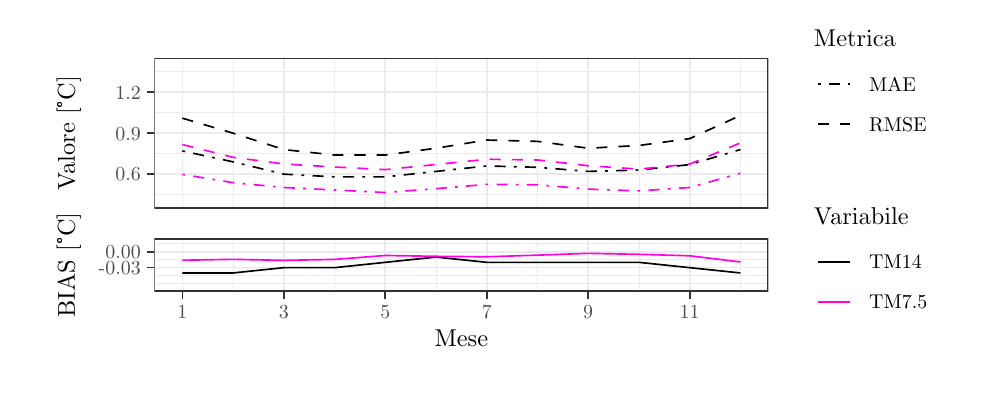
\begin{tikzpicture}[x=1pt,y=1pt]
\definecolor{fillColor}{RGB}{255,255,255}
\path[use as bounding box,fill=fillColor] (0,0) rectangle (341.43,128.04);
\begin{scope}
\path[clip] (  0.00,  0.00) rectangle (341.43,128.04);
\definecolor{drawColor}{RGB}{255,255,255}

\path[draw=drawColor,line width= 0.6pt,line join=round,line cap=round,fill=fillColor] ( -0.00,  0.00) rectangle (341.43,128.04);
\end{scope}
\begin{scope}
\path[clip] (  5.50, 57.28) rectangle (335.93,122.54);
\definecolor{drawColor}{RGB}{255,255,255}
\definecolor{fillColor}{RGB}{255,255,255}

\path[draw=drawColor,line width= 0.6pt,line join=round,line cap=round,fill=fillColor] (  5.50, 57.28) rectangle (335.93,122.54);
\end{scope}
\begin{scope}
\path[clip] (  5.50,  5.50) rectangle (335.93, 57.28);
\definecolor{drawColor}{RGB}{255,255,255}
\definecolor{fillColor}{RGB}{255,255,255}

\path[draw=drawColor,line width= 0.6pt,line join=round,line cap=round,fill=fillColor] (  5.50,  5.50) rectangle (335.93, 57.28);
\end{scope}
\begin{scope}
\path[clip] ( 45.82, 62.78) rectangle (267.62,117.04);
\definecolor{fillColor}{RGB}{255,255,255}

\path[fill=fillColor] ( 45.82, 62.78) rectangle (267.62,117.04);
\definecolor{drawColor}{gray}{0.92}

\path[draw=drawColor,line width= 0.3pt,line join=round] ( 45.82, 67.71) --
	(267.62, 67.71);

\path[draw=drawColor,line width= 0.3pt,line join=round] ( 45.82, 82.51) --
	(267.62, 82.51);

\path[draw=drawColor,line width= 0.3pt,line join=round] ( 45.82, 97.31) --
	(267.62, 97.31);

\path[draw=drawColor,line width= 0.3pt,line join=round] ( 45.82,112.10) --
	(267.62,112.10);

\path[draw=drawColor,line width= 0.3pt,line join=round] ( 74.23, 62.78) --
	( 74.23,117.04);

\path[draw=drawColor,line width= 0.3pt,line join=round] (110.89, 62.78) --
	(110.89,117.04);

\path[draw=drawColor,line width= 0.3pt,line join=round] (147.56, 62.78) --
	(147.56,117.04);

\path[draw=drawColor,line width= 0.3pt,line join=round] (184.22, 62.78) --
	(184.22,117.04);

\path[draw=drawColor,line width= 0.3pt,line join=round] (220.88, 62.78) --
	(220.88,117.04);

\path[draw=drawColor,line width= 0.3pt,line join=round] (257.54, 62.78) --
	(257.54,117.04);

\path[draw=drawColor,line width= 0.6pt,line join=round] ( 45.82, 75.11) --
	(267.62, 75.11);

\path[draw=drawColor,line width= 0.6pt,line join=round] ( 45.82, 89.91) --
	(267.62, 89.91);

\path[draw=drawColor,line width= 0.6pt,line join=round] ( 45.82,104.71) --
	(267.62,104.71);

\path[draw=drawColor,line width= 0.6pt,line join=round] ( 55.90, 62.78) --
	( 55.90,117.04);

\path[draw=drawColor,line width= 0.6pt,line join=round] ( 92.56, 62.78) --
	( 92.56,117.04);

\path[draw=drawColor,line width= 0.6pt,line join=round] (129.22, 62.78) --
	(129.22,117.04);

\path[draw=drawColor,line width= 0.6pt,line join=round] (165.89, 62.78) --
	(165.89,117.04);

\path[draw=drawColor,line width= 0.6pt,line join=round] (202.55, 62.78) --
	(202.55,117.04);

\path[draw=drawColor,line width= 0.6pt,line join=round] (239.21, 62.78) --
	(239.21,117.04);
\definecolor{drawColor}{RGB}{0,0,0}

\path[draw=drawColor,line width= 0.6pt,dash pattern=on 1pt off 3pt on 4pt off 3pt ,line join=round] ( 55.90, 83.50) --
	( 74.23, 79.55) --
	( 92.56, 75.11) --
	(110.89, 74.12) --
	(129.22, 74.12) --
	(147.56, 76.10) --
	(165.89, 78.07) --
	(184.22, 77.58) --
	(202.55, 76.10) --
	(220.88, 76.59) --
	(239.21, 78.56) --
	(257.54, 83.99);

\path[draw=drawColor,line width= 0.6pt,dash pattern=on 4pt off 4pt ,line join=round] ( 55.90, 95.33) --
	( 74.23, 89.91) --
	( 92.56, 83.99) --
	(110.89, 82.02) --
	(129.22, 82.02) --
	(147.56, 84.48) --
	(165.89, 87.44) --
	(184.22, 86.95) --
	(202.55, 84.48) --
	(220.88, 85.47) --
	(239.21, 87.94) --
	(257.54, 96.32);
\definecolor{drawColor}{RGB}{255,0,230}

\path[draw=drawColor,line width= 0.6pt,dash pattern=on 1pt off 3pt on 4pt off 3pt ,line join=round] ( 55.90, 75.01) --
	( 74.23, 72.04) --
	( 92.56, 70.28) --
	(110.89, 69.39) --
	(129.22, 68.46) --
	(147.56, 69.87) --
	(165.89, 71.42) --
	(184.22, 71.27) --
	(202.55, 69.71) --
	(220.88, 69.06) --
	(239.21, 70.29) --
	(257.54, 75.43);

\path[draw=drawColor,line width= 0.6pt,dash pattern=on 4pt off 4pt ,line join=round] ( 55.90, 85.81) --
	( 74.23, 81.19) --
	( 92.56, 78.78) --
	(110.89, 77.69) --
	(129.22, 76.75) --
	(147.56, 78.60) --
	(165.89, 80.49) --
	(184.22, 80.24) --
	(202.55, 78.15) --
	(220.88, 76.93) --
	(239.21, 78.75) --
	(257.54, 86.39);
\definecolor{drawColor}{gray}{0.20}

\path[draw=drawColor,line width= 0.6pt,line join=round,line cap=round] ( 45.82, 62.78) rectangle (267.62,117.04);
\end{scope}
\begin{scope}
\path[clip] (  0.00,  0.00) rectangle (341.43,128.04);
\definecolor{drawColor}{gray}{0.30}

\node[text=drawColor,anchor=base east,inner sep=0pt, outer sep=0pt, scale=  0.72] at ( 40.87, 72.65) {0.6};

\node[text=drawColor,anchor=base east,inner sep=0pt, outer sep=0pt, scale=  0.72] at ( 40.87, 87.45) {0.9};

\node[text=drawColor,anchor=base east,inner sep=0pt, outer sep=0pt, scale=  0.72] at ( 40.87,102.24) {1.2};
\end{scope}
\begin{scope}
\path[clip] (  0.00,  0.00) rectangle (341.43,128.04);
\definecolor{drawColor}{gray}{0.20}

\path[draw=drawColor,line width= 0.6pt,line join=round] ( 43.07, 75.11) --
	( 45.82, 75.11);

\path[draw=drawColor,line width= 0.6pt,line join=round] ( 43.07, 89.91) --
	( 45.82, 89.91);

\path[draw=drawColor,line width= 0.6pt,line join=round] ( 43.07,104.71) --
	( 45.82,104.71);
\end{scope}
\begin{scope}
\path[clip] (  0.00,  0.00) rectangle (341.43,128.04);
\definecolor{drawColor}{RGB}{0,0,0}

\node[text=drawColor,rotate= 90.00,anchor=base,inner sep=0pt, outer sep=0pt, scale=  0.88] at ( 17.06, 89.91) {Valore [\textdegree C]};
\end{scope}
\begin{scope}
\path[clip] ( 45.82, 32.79) rectangle (267.62, 51.78);
\definecolor{fillColor}{RGB}{255,255,255}

\path[fill=fillColor] ( 45.82, 32.79) rectangle (267.62, 51.78);
\definecolor{drawColor}{gray}{0.92}

\path[draw=drawColor,line width= 0.3pt,line join=round] ( 45.82, 35.57) --
	(267.62, 35.57);

\path[draw=drawColor,line width= 0.3pt,line join=round] ( 45.82, 38.45) --
	(267.62, 38.45);

\path[draw=drawColor,line width= 0.3pt,line join=round] ( 45.82, 44.20) --
	(267.62, 44.20);

\path[draw=drawColor,line width= 0.3pt,line join=round] ( 45.82, 49.96) --
	(267.62, 49.96);

\path[draw=drawColor,line width= 0.3pt,line join=round] ( 74.23, 32.79) --
	( 74.23, 51.78);

\path[draw=drawColor,line width= 0.3pt,line join=round] (110.89, 32.79) --
	(110.89, 51.78);

\path[draw=drawColor,line width= 0.3pt,line join=round] (147.56, 32.79) --
	(147.56, 51.78);

\path[draw=drawColor,line width= 0.3pt,line join=round] (184.22, 32.79) --
	(184.22, 51.78);

\path[draw=drawColor,line width= 0.3pt,line join=round] (220.88, 32.79) --
	(220.88, 51.78);

\path[draw=drawColor,line width= 0.3pt,line join=round] (257.54, 32.79) --
	(257.54, 51.78);

\path[draw=drawColor,line width= 0.6pt,line join=round] ( 45.82, 41.32) --
	(267.62, 41.32);

\path[draw=drawColor,line width= 0.6pt,line join=round] ( 45.82, 47.08) --
	(267.62, 47.08);

\path[draw=drawColor,line width= 0.6pt,line join=round] ( 55.90, 32.79) --
	( 55.90, 51.78);

\path[draw=drawColor,line width= 0.6pt,line join=round] ( 92.56, 32.79) --
	( 92.56, 51.78);

\path[draw=drawColor,line width= 0.6pt,line join=round] (129.22, 32.79) --
	(129.22, 51.78);

\path[draw=drawColor,line width= 0.6pt,line join=round] (165.89, 32.79) --
	(165.89, 51.78);

\path[draw=drawColor,line width= 0.6pt,line join=round] (202.55, 32.79) --
	(202.55, 51.78);

\path[draw=drawColor,line width= 0.6pt,line join=round] (239.21, 32.79) --
	(239.21, 51.78);
\definecolor{drawColor}{RGB}{0,0,0}

\path[draw=drawColor,line width= 0.6pt,line join=round] ( 55.90, 39.41) --
	( 74.23, 39.41) --
	( 92.56, 41.32) --
	(110.89, 41.32) --
	(129.22, 43.24) --
	(147.56, 45.16) --
	(165.89, 43.24) --
	(184.22, 43.24) --
	(202.55, 43.24) --
	(220.88, 43.24) --
	(239.21, 41.32) --
	(257.54, 39.41);
\definecolor{drawColor}{RGB}{255,0,230}

\path[draw=drawColor,line width= 0.6pt,line join=round] ( 55.90, 44.01) --
	( 74.23, 44.33) --
	( 92.56, 43.96) --
	(110.89, 44.30) --
	(129.22, 45.72) --
	(147.56, 45.42) --
	(165.89, 45.25) --
	(184.22, 45.84) --
	(202.55, 46.49) --
	(220.88, 46.14) --
	(239.21, 45.61) --
	(257.54, 43.38);
\definecolor{drawColor}{gray}{0.20}

\path[draw=drawColor,line width= 0.6pt,line join=round,line cap=round] ( 45.82, 32.79) rectangle (267.62, 51.78);
\end{scope}
\begin{scope}
\path[clip] (  0.00,  0.00) rectangle (341.43,128.04);
\definecolor{drawColor}{gray}{0.30}

\node[text=drawColor,anchor=base east,inner sep=0pt, outer sep=0pt, scale=  0.72] at ( 40.87, 38.86) {-0.03};

\node[text=drawColor,anchor=base east,inner sep=0pt, outer sep=0pt, scale=  0.72] at ( 40.87, 44.62) {0.00};
\end{scope}
\begin{scope}
\path[clip] (  0.00,  0.00) rectangle (341.43,128.04);
\definecolor{drawColor}{gray}{0.20}

\path[draw=drawColor,line width= 0.6pt,line join=round] ( 43.07, 41.32) --
	( 45.82, 41.32);

\path[draw=drawColor,line width= 0.6pt,line join=round] ( 43.07, 47.08) --
	( 45.82, 47.08);
\end{scope}
\begin{scope}
\path[clip] (  0.00,  0.00) rectangle (341.43,128.04);
\definecolor{drawColor}{gray}{0.20}

\path[draw=drawColor,line width= 0.6pt,line join=round] ( 55.90, 30.04) --
	( 55.90, 32.79);

\path[draw=drawColor,line width= 0.6pt,line join=round] ( 92.56, 30.04) --
	( 92.56, 32.79);

\path[draw=drawColor,line width= 0.6pt,line join=round] (129.22, 30.04) --
	(129.22, 32.79);

\path[draw=drawColor,line width= 0.6pt,line join=round] (165.89, 30.04) --
	(165.89, 32.79);

\path[draw=drawColor,line width= 0.6pt,line join=round] (202.55, 30.04) --
	(202.55, 32.79);

\path[draw=drawColor,line width= 0.6pt,line join=round] (239.21, 30.04) --
	(239.21, 32.79);
\end{scope}
\begin{scope}
\path[clip] (  0.00,  0.00) rectangle (341.43,128.04);
\definecolor{drawColor}{gray}{0.30}

\node[text=drawColor,anchor=base,inner sep=0pt, outer sep=0pt, scale=  0.72] at ( 55.90, 22.91) {1};

\node[text=drawColor,anchor=base,inner sep=0pt, outer sep=0pt, scale=  0.72] at ( 92.56, 22.91) {3};

\node[text=drawColor,anchor=base,inner sep=0pt, outer sep=0pt, scale=  0.72] at (129.22, 22.91) {5};

\node[text=drawColor,anchor=base,inner sep=0pt, outer sep=0pt, scale=  0.72] at (165.89, 22.91) {7};

\node[text=drawColor,anchor=base,inner sep=0pt, outer sep=0pt, scale=  0.72] at (202.55, 22.91) {9};

\node[text=drawColor,anchor=base,inner sep=0pt, outer sep=0pt, scale=  0.72] at (239.21, 22.91) {11};
\end{scope}
\begin{scope}
\path[clip] (  0.00,  0.00) rectangle (341.43,128.04);
\definecolor{drawColor}{RGB}{0,0,0}

\node[text=drawColor,anchor=base,inner sep=0pt, outer sep=0pt, scale=  0.88] at (156.72, 12.71) {Mese};
\end{scope}
\begin{scope}
\path[clip] (  0.00,  0.00) rectangle (341.43,128.04);
\definecolor{drawColor}{RGB}{0,0,0}

\node[text=drawColor,rotate= 90.00,anchor=base,inner sep=0pt, outer sep=0pt, scale=  0.88] at ( 17.06, 42.28) {BIAS [\textdegree C]};
\end{scope}
\begin{scope}
\path[clip] (  0.00,  0.00) rectangle (341.43,128.04);
\definecolor{fillColor}{RGB}{255,255,255}

\path[fill=fillColor] (278.62, 80.41) rectangle (330.23,133.59);
\end{scope}
\begin{scope}
\path[clip] (  0.00,  0.00) rectangle (341.43,128.04);
\definecolor{drawColor}{RGB}{0,0,0}

\node[text=drawColor,anchor=base west,inner sep=0pt, outer sep=0pt, scale=  0.88] at (284.12,121.18) {Metrica};
\end{scope}
\begin{scope}
\path[clip] (  0.00,  0.00) rectangle (341.43,128.04);
\definecolor{fillColor}{RGB}{255,255,255}

\path[fill=fillColor] (284.12,100.37) rectangle (298.58,114.82);
\end{scope}
\begin{scope}
\path[clip] (  0.00,  0.00) rectangle (341.43,128.04);
\definecolor{drawColor}{RGB}{0,0,0}

\path[draw=drawColor,line width= 0.6pt,dash pattern=on 1pt off 3pt on 4pt off 3pt ,line join=round] (285.57,107.59) -- (297.13,107.59);
\end{scope}
\begin{scope}
\path[clip] (  0.00,  0.00) rectangle (341.43,128.04);
\definecolor{fillColor}{RGB}{255,255,255}

\path[fill=fillColor] (284.12, 85.91) rectangle (298.58,100.37);
\end{scope}
\begin{scope}
\path[clip] (  0.00,  0.00) rectangle (341.43,128.04);
\definecolor{drawColor}{RGB}{0,0,0}

\path[draw=drawColor,line width= 0.6pt,dash pattern=on 4pt off 4pt ,line join=round] (285.57, 93.14) -- (297.13, 93.14);
\end{scope}
\begin{scope}
\path[clip] (  0.00,  0.00) rectangle (341.43,128.04);
\definecolor{drawColor}{RGB}{0,0,0}

\node[text=drawColor,anchor=base west,inner sep=0pt, outer sep=0pt, scale=  0.72] at (304.08,105.13) {MAE};
\end{scope}
\begin{scope}
\path[clip] (  0.00,  0.00) rectangle (341.43,128.04);
\definecolor{drawColor}{RGB}{0,0,0}

\node[text=drawColor,anchor=base west,inner sep=0pt, outer sep=0pt, scale=  0.72] at (304.08, 90.68) {RMSE};
\end{scope}
\begin{scope}
\path[clip] (  0.00,  0.00) rectangle (341.43,128.04);
\definecolor{fillColor}{RGB}{255,255,255}

\path[fill=fillColor] (278.62, 16.23) rectangle (330.43, 69.41);
\end{scope}
\begin{scope}
\path[clip] (  0.00,  0.00) rectangle (341.43,128.04);
\definecolor{drawColor}{RGB}{0,0,0}

\node[text=drawColor,anchor=base west,inner sep=0pt, outer sep=0pt, scale=  0.88] at (284.12, 57.00) {Variabile};
\end{scope}
\begin{scope}
\path[clip] (  0.00,  0.00) rectangle (341.43,128.04);
\definecolor{fillColor}{RGB}{255,255,255}

\path[fill=fillColor] (284.12, 36.19) rectangle (298.58, 50.64);
\end{scope}
\begin{scope}
\path[clip] (  0.00,  0.00) rectangle (341.43,128.04);
\definecolor{drawColor}{RGB}{0,0,0}

\path[draw=drawColor,line width= 0.6pt,line join=round] (285.57, 43.41) -- (297.13, 43.41);
\end{scope}
\begin{scope}
\path[clip] (  0.00,  0.00) rectangle (341.43,128.04);
\definecolor{fillColor}{RGB}{255,255,255}

\path[fill=fillColor] (284.12, 21.73) rectangle (298.58, 36.19);
\end{scope}
\begin{scope}
\path[clip] (  0.00,  0.00) rectangle (341.43,128.04);
\definecolor{drawColor}{RGB}{255,0,230}

\path[draw=drawColor,line width= 0.6pt,line join=round] (285.57, 28.96) -- (297.13, 28.96);
\end{scope}
\begin{scope}
\path[clip] (  0.00,  0.00) rectangle (341.43,128.04);
\definecolor{drawColor}{RGB}{0,0,0}

\node[text=drawColor,anchor=base west,inner sep=0pt, outer sep=0pt, scale=  0.72] at (304.08, 40.95) {TM14};
\end{scope}
\begin{scope}
\path[clip] (  0.00,  0.00) rectangle (341.43,128.04);
\definecolor{drawColor}{RGB}{0,0,0}

\node[text=drawColor,anchor=base west,inner sep=0pt, outer sep=0pt, scale=  0.72] at (304.08, 26.50) {TM7.5};
\end{scope}
\end{tikzpicture}
